\chapter{Практическая часть}
\section{Текст программы}
\lstset{language=matlab}

В листинге~\ref{lst:programm} приведён текст программы.
\begin{lstlisting}[caption={Текст программы},label={lst:programm}]
function lab1()
    X=[
        -2.79, -3.01, -4.07, -2.85, -2.43, -3.20, ...
        -3.72, -4.27, -5.48, -2.38, -4.69, -4.34, ...
        -5.08, -5.01, -4.08, -4.20, -4.74, -1.88, ...
        -3.25, -2.78, -3.56, -3.54, -3.79, -3.18, ...
        -5.08, -4.30, -2.86, -2.45, -3.08, -3.22, ...
        -2.76, -3.20, -3.33, -4.91, -4.06, -3.81, ...
        -3.96, -3.65, -3.77, -4.60, -5.21, -2.67, ...
        -1.95, -2.43, -1.73, -2.50, -3.96, -3.75, ...
        -2.70, -4.26, -3.42, -4.07, -4.74, -3.00, ...
        -4.37, -5.42, -5.00, -4.08, -2.46, -4.33, ...
        -4.08, -3.72, -4.09, -2.96, -3.71, -1.51, ...
        -3.70, -6.48, -4.26, -4.39, -3.16, -4.63, ...
        -2.66, -2.22, -4.79, -2.46, -3.69, -3.35, ...
        -2.32, -4.17, -3.85, -4.93, -2.05, -3.15, ...
        -3.49, -5.70, -2.53, -3.85, -4.32, -3.37, ...
        -3.98, -3.74, -5.28, -2.56, -3.21, -3.10, ...
        -3.78, -3.36, -3.32, -2.59, -2.45, -3.34, ...
        -3.20, -4.14, -4.00, -4.79, -4.02, -4.58, ...
        -4.45, -3.69, -4.53, -3.98, -4.51, -4.44, ...
        -3.78, -4.24, -4.00, -2.46, -2.58, -4.04, ...
    ];
    X = sort(X);

    % Максимальное значение выборки
    Mmax = max(X);
    % Минимальное значение выборки
    Mmin = min(X);

    % Разброс выборки
    R = Mmax - Mmin;

    % Оценка мат. ожидания
    mu = mean(X);
    % Оценка дисперсии
    D = var(X);

    fprintf('Mmax = %f\n', Mmax);
    fprintf('Mmin = %f\n', Mmin);
    fprintf('R = %f\n', R);
    fprintf('Mean = %f\n', mu);
    fprintf('Varience = %f\n\n', D);

    % Нахождение количества интервалов
    m = floor(log2(length(X))) + 2;
    % Группировка значений в m интервалов
    [N, edges] = histcounts(X, m, 'BinLimits', [Mmin, Mmax]);
    len_c = length(N);

    % Вывод всех интервалов и количества элементов
    fprintf('%d intervals:\n', m);
    for i = 1 : (len_c - 1)
        fprintf('[%f,%f) - %d\n', edges(i), edges(i + 1), N(i));
    end
    fprintf('[%f,%f] - %d\n', edges(len_c), edges(len_c + 1), N(len_c));

    % График функции плотности распределения вероятностей нормальной 
    % случайной величины
    f = normpdf(X, mu, sqrt(D));
    % Построение гистограммы
    histogram(X, m, 'Normalization', 'pdf', 'BinLimits', [Mmin, Mmax]);
    % Построение на одной координатной плоскости
    hold on;
    % Построение графика функции плотности распределения
    plot(X, f, 'LineWidth', 2);
    legend({'Гистограмма', 'Функция плотности распределения'}, ...
        'Location','northwest');
    % Новая координатная плоскость
    figure;
    % График функции распределения нормальной случайной величины
    F = normcdf(X, mu, sqrt(D));
    % Построение графика эмпирической функции распределения
    [YY, XX] = ecdf(X);
    stairs(XX, YY, 'LineWidth', 2);
    hold on;
    % Построение графика функции распределения
    plot(X, F, 'LineWidth', 2);
    legend({'Эмперическая функция распределения', ...
        'Функция распределения'}, ...
        'Location','northwest');
end
\end{lstlisting}

\section{Результат}

В листинге~\ref{lst:result} приведён результат выполнения описанной программы.
\begin{lstlisting}[language=,numbers=none,caption={Результат программы},label={lst:result}]
Mmax = -1.510000
Mmin = -6.480000
R = 4.970000
Mean = -3.676167
Varience = 0.866410

8 intervals:
[-6.480000,-5.858750) - 1
[-5.858750,-5.237500) - 4
[-5.237500,-4.616250) - 13
[-4.616250,-3.995000) - 30
[-3.995000,-3.373750) - 24
[-3.373750,-2.752500) - 25
[-2.752500,-2.131250) - 18
[-2.131250,-1.510000] - 5\end{lstlisting}

На рисунке \ref{img:plot01} представлена гистограмма и график функции плотности распределения вероятностей нормальной случайной величины с математическим ожиданием $\hat \mu$ и дисперсией $S^2$
\begin{figure}[H]
    \centering
    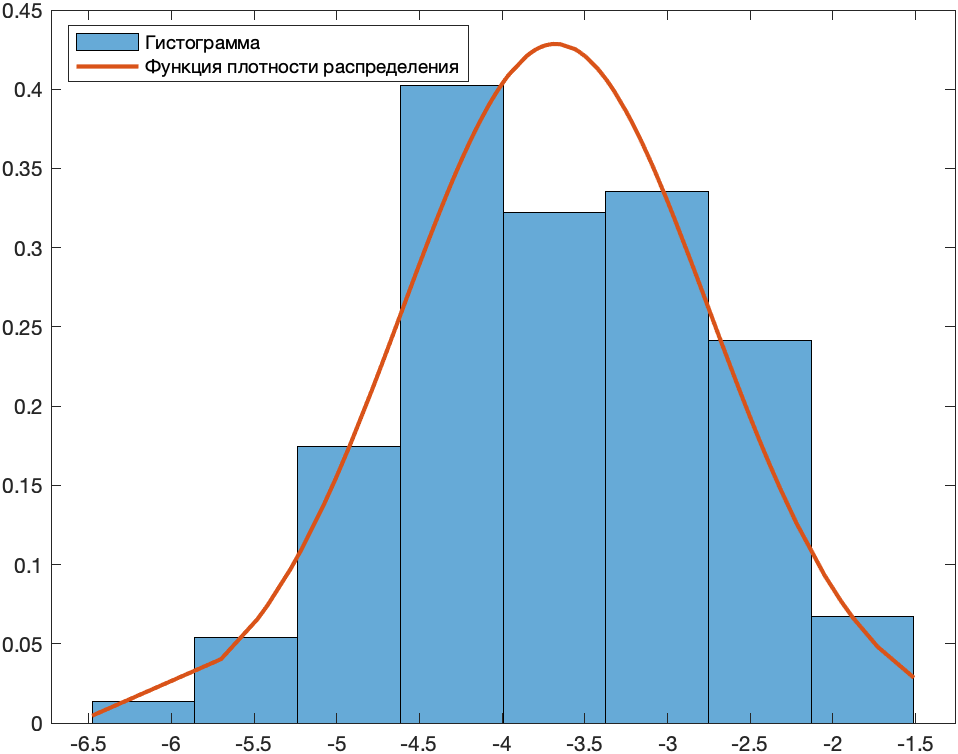
\includegraphics[scale=1]{plots/1.png}
    \caption{}
    \label{img:plot01}
\end{figure}

На рисунке \ref{img:plot02} представлены графики эмпирической функции распределения и функции распределения нормальной случайной величины с математическим ожиданием $\hat \mu$ и дисперсией $S^2$
\begin{figure}[H]
    \centering
    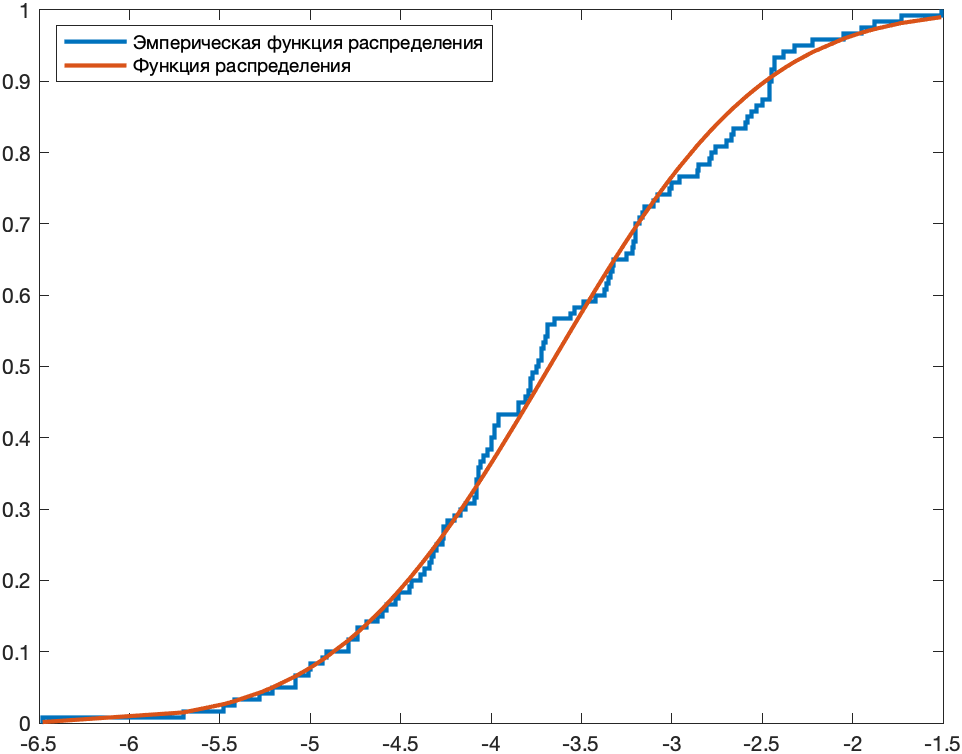
\includegraphics[scale=1]{plots/2.png}
    \caption{}
    \label{img:plot02}
\end{figure}

%\begin{figure}[H]
    %\caption{Гистограмма и график функции плотности распределения вероятностей нормальной случайной величины с математическим ожиданием $\hat \mu$ и дисперсией $S^2$}\label{img:plot01}

    %\input{plots/untitled3.pdf}
%\end{figure}

%\begin{figure}[H]
    %\caption{График эмпирической функции распределения и функции распределения нормальной случайной величины с математическим ожиданием $\hat \mu$ и дисперсией $S^2$}\label{img:plot02}
    %\input{plots/untitled4.pdf}
%\end{figure}

